% Options for packages loaded elsewhere
\PassOptionsToPackage{unicode}{hyperref}
\PassOptionsToPackage{hyphens}{url}
%
\documentclass[
]{article}
\usepackage{amsmath,amssymb}
\usepackage{iftex}
\ifPDFTeX
  \usepackage[T1]{fontenc}
  \usepackage[utf8]{inputenc}
  \usepackage{textcomp} % provide euro and other symbols
\else % if luatex or xetex
  \usepackage{unicode-math} % this also loads fontspec
  \defaultfontfeatures{Scale=MatchLowercase}
  \defaultfontfeatures[\rmfamily]{Ligatures=TeX,Scale=1}
\fi
\usepackage{lmodern}
\ifPDFTeX\else
  % xetex/luatex font selection
\fi
% Use upquote if available, for straight quotes in verbatim environments
\IfFileExists{upquote.sty}{\usepackage{upquote}}{}
\IfFileExists{microtype.sty}{% use microtype if available
  \usepackage[]{microtype}
  \UseMicrotypeSet[protrusion]{basicmath} % disable protrusion for tt fonts
}{}
\makeatletter
\@ifundefined{KOMAClassName}{% if non-KOMA class
  \IfFileExists{parskip.sty}{%
    \usepackage{parskip}
  }{% else
    \setlength{\parindent}{0pt}
    \setlength{\parskip}{6pt plus 2pt minus 1pt}}
}{% if KOMA class
  \KOMAoptions{parskip=half}}
\makeatother
\usepackage{xcolor}
\usepackage[margin=1in]{geometry}
\usepackage{color}
\usepackage{fancyvrb}
\newcommand{\VerbBar}{|}
\newcommand{\VERB}{\Verb[commandchars=\\\{\}]}
\DefineVerbatimEnvironment{Highlighting}{Verbatim}{commandchars=\\\{\}}
% Add ',fontsize=\small' for more characters per line
\usepackage{framed}
\definecolor{shadecolor}{RGB}{248,248,248}
\newenvironment{Shaded}{\begin{snugshade}}{\end{snugshade}}
\newcommand{\AlertTok}[1]{\textcolor[rgb]{0.94,0.16,0.16}{#1}}
\newcommand{\AnnotationTok}[1]{\textcolor[rgb]{0.56,0.35,0.01}{\textbf{\textit{#1}}}}
\newcommand{\AttributeTok}[1]{\textcolor[rgb]{0.13,0.29,0.53}{#1}}
\newcommand{\BaseNTok}[1]{\textcolor[rgb]{0.00,0.00,0.81}{#1}}
\newcommand{\BuiltInTok}[1]{#1}
\newcommand{\CharTok}[1]{\textcolor[rgb]{0.31,0.60,0.02}{#1}}
\newcommand{\CommentTok}[1]{\textcolor[rgb]{0.56,0.35,0.01}{\textit{#1}}}
\newcommand{\CommentVarTok}[1]{\textcolor[rgb]{0.56,0.35,0.01}{\textbf{\textit{#1}}}}
\newcommand{\ConstantTok}[1]{\textcolor[rgb]{0.56,0.35,0.01}{#1}}
\newcommand{\ControlFlowTok}[1]{\textcolor[rgb]{0.13,0.29,0.53}{\textbf{#1}}}
\newcommand{\DataTypeTok}[1]{\textcolor[rgb]{0.13,0.29,0.53}{#1}}
\newcommand{\DecValTok}[1]{\textcolor[rgb]{0.00,0.00,0.81}{#1}}
\newcommand{\DocumentationTok}[1]{\textcolor[rgb]{0.56,0.35,0.01}{\textbf{\textit{#1}}}}
\newcommand{\ErrorTok}[1]{\textcolor[rgb]{0.64,0.00,0.00}{\textbf{#1}}}
\newcommand{\ExtensionTok}[1]{#1}
\newcommand{\FloatTok}[1]{\textcolor[rgb]{0.00,0.00,0.81}{#1}}
\newcommand{\FunctionTok}[1]{\textcolor[rgb]{0.13,0.29,0.53}{\textbf{#1}}}
\newcommand{\ImportTok}[1]{#1}
\newcommand{\InformationTok}[1]{\textcolor[rgb]{0.56,0.35,0.01}{\textbf{\textit{#1}}}}
\newcommand{\KeywordTok}[1]{\textcolor[rgb]{0.13,0.29,0.53}{\textbf{#1}}}
\newcommand{\NormalTok}[1]{#1}
\newcommand{\OperatorTok}[1]{\textcolor[rgb]{0.81,0.36,0.00}{\textbf{#1}}}
\newcommand{\OtherTok}[1]{\textcolor[rgb]{0.56,0.35,0.01}{#1}}
\newcommand{\PreprocessorTok}[1]{\textcolor[rgb]{0.56,0.35,0.01}{\textit{#1}}}
\newcommand{\RegionMarkerTok}[1]{#1}
\newcommand{\SpecialCharTok}[1]{\textcolor[rgb]{0.81,0.36,0.00}{\textbf{#1}}}
\newcommand{\SpecialStringTok}[1]{\textcolor[rgb]{0.31,0.60,0.02}{#1}}
\newcommand{\StringTok}[1]{\textcolor[rgb]{0.31,0.60,0.02}{#1}}
\newcommand{\VariableTok}[1]{\textcolor[rgb]{0.00,0.00,0.00}{#1}}
\newcommand{\VerbatimStringTok}[1]{\textcolor[rgb]{0.31,0.60,0.02}{#1}}
\newcommand{\WarningTok}[1]{\textcolor[rgb]{0.56,0.35,0.01}{\textbf{\textit{#1}}}}
\usepackage{graphicx}
\makeatletter
\def\maxwidth{\ifdim\Gin@nat@width>\linewidth\linewidth\else\Gin@nat@width\fi}
\def\maxheight{\ifdim\Gin@nat@height>\textheight\textheight\else\Gin@nat@height\fi}
\makeatother
% Scale images if necessary, so that they will not overflow the page
% margins by default, and it is still possible to overwrite the defaults
% using explicit options in \includegraphics[width, height, ...]{}
\setkeys{Gin}{width=\maxwidth,height=\maxheight,keepaspectratio}
% Set default figure placement to htbp
\makeatletter
\def\fps@figure{htbp}
\makeatother
\setlength{\emergencystretch}{3em} % prevent overfull lines
\providecommand{\tightlist}{%
  \setlength{\itemsep}{0pt}\setlength{\parskip}{0pt}}
\setcounter{secnumdepth}{-\maxdimen} % remove section numbering
\ifLuaTeX
  \usepackage{selnolig}  % disable illegal ligatures
\fi
\usepackage{bookmark}
\IfFileExists{xurl.sty}{\usepackage{xurl}}{} % add URL line breaks if available
\urlstyle{same}
\hypersetup{
  pdftitle={Lab 7: Networks},
  pdfauthor={Lauren Ponisio},
  hidelinks,
  pdfcreator={LaTeX via pandoc}}

\title{Lab 7: Networks}
\author{Lauren Ponisio}
\date{}

\begin{document}
\maketitle

\section{Computational Topics}\label{computational-topics}

\begin{itemize}
\tightlist
\item
  Build and visualize food webs
\item
  Write functions to implement mathematical equations
\end{itemize}

\section{Conservation topics}\label{conservation-topics}

\begin{itemize}
\tightlist
\item
  Paleofood webs
\item
  Species extinction
\end{itemize}

In this lab we will practice our network visualization and manipulation
skills using the paleo food web data from
\href{https://doi.org/10.1073/pnas.1408471111}{Yeakel et al.~2014}.

\begin{figure}
\centering
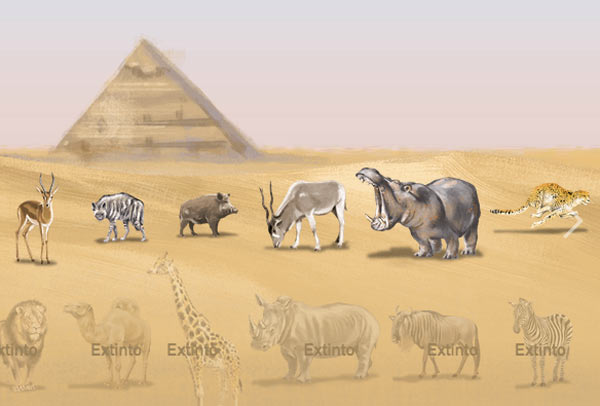
\includegraphics{figures/paleoweb.jpg}
\caption{Paleoweb}
\end{figure}

See the beautiful, animated version of the graphic above
\href{https://infograficos.estadao.com.br/public/cidades/extincoes-egito/}{here}

With some interaction networks we can observe the interactions, for
example plant-pollinator networks, seed-disperal networks, human social
networks. In food webs sometimes feeding interactions are observed
directly, through camera traps, people doing timed observations, and now
molecular analysis of gut contents/scat. However, often with food webs
people build probabilistic models of who interacts with who based on
body size (as in the Yeakel et al.~2014), especially with paleowebs.
Thus the data from Yeakel et al.~is 1) an occurrence matrix (Figure 2
from the publication) and a matrix of body sizes (two columns, females
then males). We will use these data to build the foodwebs for each time
period. This lab is pretty challenging because it will use many of our
core programming skills (for loops, writing functions, subsetting data)
and our network skills.

First we will read in the data. The matrix we are reading in has no row
or column names, we will have to set them.

\begin{Shaded}
\begin{Highlighting}[]
\NormalTok{sp\_occ }\OtherTok{\textless{}{-}} \FunctionTok{read.table}\NormalTok{(}\AttributeTok{file=}\StringTok{"data/egypt\_data.txt"}\NormalTok{, }\AttributeTok{header =} \ConstantTok{FALSE}\NormalTok{)}
\FunctionTok{str}\NormalTok{(sp\_occ)}
\end{Highlighting}
\end{Shaded}

\begin{verbatim}
## 'data.frame':    39 obs. of  23 variables:
##  $ V1 : int  1 1 1 1 1 1 1 1 0 1 ...
##  $ V2 : int  1 1 1 1 1 1 1 1 0 1 ...
##  $ V3 : int  1 1 1 1 0 1 1 1 0 1 ...
##  $ V4 : int  1 1 1 1 0 1 1 1 0 1 ...
##  $ V5 : int  1 1 1 1 0 1 1 1 0 1 ...
##  $ V6 : int  1 1 1 1 0 1 1 1 0 1 ...
##  $ V7 : int  1 1 1 1 0 1 1 1 0 1 ...
##  $ V8 : int  1 1 1 1 0 0 1 1 0 1 ...
##  $ V9 : int  1 1 1 1 0 0 1 1 0 0 ...
##  $ V10: int  1 1 1 1 0 0 1 1 0 0 ...
##  $ V11: int  1 1 1 1 0 0 1 1 0 0 ...
##  $ V12: int  1 1 1 1 0 0 1 1 1 0 ...
##  $ V13: int  1 1 1 1 0 0 1 1 1 0 ...
##  $ V14: int  1 1 0 1 0 0 1 1 1 0 ...
##  $ V15: int  1 1 0 1 0 0 1 1 1 0 ...
##  $ V16: int  1 1 0 1 0 0 1 1 1 0 ...
##  $ V17: int  1 1 0 1 0 0 1 1 1 0 ...
##  $ V18: int  1 1 0 1 0 0 0 1 1 0 ...
##  $ V19: int  1 1 0 1 0 0 0 1 1 0 ...
##  $ V20: int  1 1 0 1 0 0 0 1 1 0 ...
##  $ V21: int  1 1 0 1 0 0 0 1 0 0 ...
##  $ V22: int  1 1 0 1 0 0 0 1 0 0 ...
##  $ V23: int  1 1 0 1 0 0 0 0 0 0 ...
\end{verbatim}

\begin{Shaded}
\begin{Highlighting}[]
\NormalTok{sp\_mass }\OtherTok{\textless{}{-}} \FunctionTok{read.table}\NormalTok{(}\AttributeTok{file=}\StringTok{"data/egypt\_mass.txt"}\NormalTok{, }\AttributeTok{header=}\ConstantTok{FALSE}\NormalTok{)}
\FunctionTok{str}\NormalTok{(sp\_mass)}
\end{Highlighting}
\end{Shaded}

\begin{verbatim}
## 'data.frame':    39 obs. of  2 variables:
##  $ V1: int  6 4 18 25 40 122 122 50 35 2200 ...
##  $ V2: int  15 8 36 55 90 260 260 60 65 6300 ...
\end{verbatim}

\begin{figure}
\centering
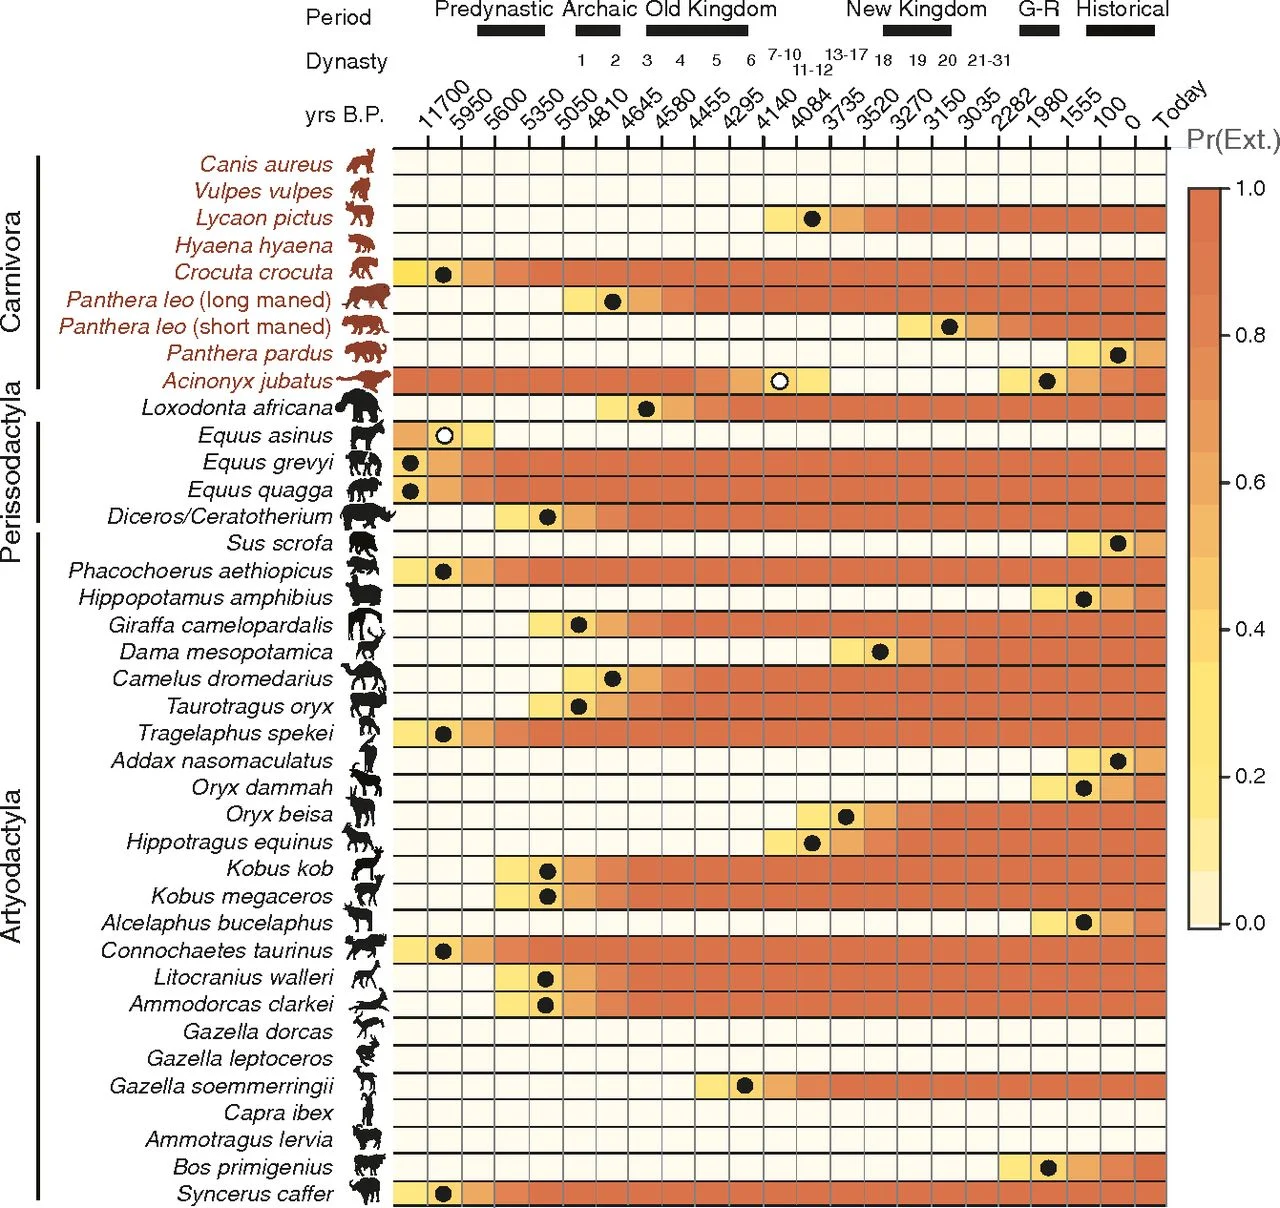
\includegraphics{figures/figure2.jpg}
\caption{Figure 2}
\end{figure}

The rows are arranged in the order of Figure 2 of the manuscript. To set
the rownames we can make a vector of the names then use the function
`rownames'. We also have to note which species are predators (all those
in the species in the Carnivora clade in figure 2). Otherwise we will
create a web where giraffes are voracious predators consuming all of the
other species (I made this mistake when constructing the networks
originally). I have transcribed the data from figure 2 for you:

\begin{Shaded}
\begin{Highlighting}[]
\NormalTok{row\_labs\_sp }\OtherTok{\textless{}{-}} \FunctionTok{c}\NormalTok{(}\StringTok{"Canis aureus"}\NormalTok{, }\StringTok{"Vulpes vulpes"}\NormalTok{, }\StringTok{"Lycaon pictus"}\NormalTok{, }\StringTok{"Hyaena hyaena"}\NormalTok{, }\StringTok{"Crocuta crocuta"}\NormalTok{, }\StringTok{"Panthera leo (long maned)"}\NormalTok{, }\StringTok{"Panthera leo (short maned)"}\NormalTok{, }\StringTok{"Panthera pardus"}\NormalTok{, }\StringTok{"Acinonyx jubatus"}\NormalTok{, }\StringTok{"Loxodonta africana"}\NormalTok{, }\StringTok{"Equus asinus"}\NormalTok{, }\StringTok{"Equus grevyi"}\NormalTok{, }\StringTok{"Equus quagga"}\NormalTok{, }\StringTok{"Diceros/Ceratotherium"}\NormalTok{, }\StringTok{"Sus scrofa"}\NormalTok{,  }\StringTok{"Phacochoerus aethiopicus"}\NormalTok{, }\StringTok{"Hippopotamus amphibius"}\NormalTok{, }\StringTok{"Giraffa camelopardalis"}\NormalTok{, }\StringTok{"Dama mesopotamica"}\NormalTok{, }\StringTok{"Camelus dromedarius"}\NormalTok{, }\StringTok{"Taurotragus oryx"}\NormalTok{, }\StringTok{"Tragelaphus spekei"}\NormalTok{, }\StringTok{"Addax nasomaculatus"}\NormalTok{, }\StringTok{"Oryx dammah"}\NormalTok{, }\StringTok{"Oryx beisa"}\NormalTok{, }\StringTok{"Hippotragus equinus"}\NormalTok{, }\StringTok{"Kobus kob"}\NormalTok{, }\StringTok{"Kobus megaceros"}\NormalTok{, }\StringTok{"Alcelaphus bucelaphus"}\NormalTok{, }\StringTok{"Connochaetes taurinus"}\NormalTok{, }\StringTok{"Litocranius walleri"}\NormalTok{, }\StringTok{"Ammodorcas clarkei"}\NormalTok{, }\StringTok{"Gazella dorcas"}\NormalTok{, }\StringTok{"Gazella leptoceros"}\NormalTok{, }\StringTok{"Gazella soemmerringii"}\NormalTok{, }\StringTok{"Capra ibex"}\NormalTok{, }\StringTok{"Ammotragus lervia"}\NormalTok{, }\StringTok{"Bos primigenius"}\NormalTok{, }\StringTok{"Syncerus caffer"}\NormalTok{)}

\DocumentationTok{\#\# Set 1 for predators, 0 for prey  }
\NormalTok{carnivores }\OtherTok{\textless{}{-}} \FunctionTok{c}\NormalTok{(}\FunctionTok{rep}\NormalTok{(}\DecValTok{1}\NormalTok{, }\DecValTok{9}\NormalTok{), }\FunctionTok{rep}\NormalTok{(}\DecValTok{0}\NormalTok{, }\FunctionTok{length}\NormalTok{(row\_labs\_sp)}\SpecialCharTok{{-}} \DecValTok{9}\NormalTok{))}
\FunctionTok{names}\NormalTok{(carnivores) }\OtherTok{\textless{}{-}}\NormalTok{ row\_labs\_sp}
\end{Highlighting}
\end{Shaded}

\section{Lab part 1: Creating our foodwebs based on body
sizes.}\label{lab-part-1-creating-our-foodwebs-based-on-body-sizes.}

\begin{enumerate}
\def\labelenumi{\alph{enumi}.}
\tightlist
\item
  Use the above vector of species names to label the row names of the
  species occurrence and the body size matrices. The columns of the
  species occurrence matrix are time points, so we can leave those as V1
  etc., but we should set the column names of the mass matrix as ``f'',
  ``m'' (female and male). Use `head' to check each matrix to see if the
  names are displayed properly.
\end{enumerate}

\begin{Shaded}
\begin{Highlighting}[]
\FunctionTok{rownames}\NormalTok{(sp\_occ) }\OtherTok{\textless{}{-}}\NormalTok{ row\_labs\_sp}
\FunctionTok{rownames}\NormalTok{(sp\_mass) }\OtherTok{\textless{}{-}}\NormalTok{ row\_labs\_sp}
\FunctionTok{colnames}\NormalTok{(sp\_mass) }\OtherTok{\textless{}{-}} \FunctionTok{c}\NormalTok{(}\StringTok{"f"}\NormalTok{, }\StringTok{"m"}\NormalTok{)}
\FunctionTok{head}\NormalTok{(sp\_occ)}
\end{Highlighting}
\end{Shaded}

\begin{verbatim}
##                           V1 V2 V3 V4 V5 V6 V7 V8 V9 V10 V11 V12 V13 V14 V15
## Canis aureus               1  1  1  1  1  1  1  1  1   1   1   1   1   1   1
## Vulpes vulpes              1  1  1  1  1  1  1  1  1   1   1   1   1   1   1
## Lycaon pictus              1  1  1  1  1  1  1  1  1   1   1   1   1   0   0
## Hyaena hyaena              1  1  1  1  1  1  1  1  1   1   1   1   1   1   1
## Crocuta crocuta            1  1  0  0  0  0  0  0  0   0   0   0   0   0   0
## Panthera leo (long maned)  1  1  1  1  1  1  1  0  0   0   0   0   0   0   0
##                           V16 V17 V18 V19 V20 V21 V22 V23
## Canis aureus                1   1   1   1   1   1   1   1
## Vulpes vulpes               1   1   1   1   1   1   1   1
## Lycaon pictus               0   0   0   0   0   0   0   0
## Hyaena hyaena               1   1   1   1   1   1   1   1
## Crocuta crocuta             0   0   0   0   0   0   0   0
## Panthera leo (long maned)   0   0   0   0   0   0   0   0
\end{verbatim}

\begin{Shaded}
\begin{Highlighting}[]
\FunctionTok{head}\NormalTok{(sp\_mass)}
\end{Highlighting}
\end{Shaded}

\begin{verbatim}
##                             f   m
## Canis aureus                6  15
## Vulpes vulpes               4   8
## Lycaon pictus              18  36
## Hyaena hyaena              25  55
## Crocuta crocuta            40  90
## Panthera leo (long maned) 122 260
\end{verbatim}

Yeakel recommended an updated equation to estimate the probability a
predator consumed a prey based on their relative body masses from
\href{https://doi.org/10.1086/653667}{Rohr et al.~2010.}. The
probability of existence of a trophic link between a predator of
body-size \(m_i\) and a prey of body-size \(m_j\) is given by:

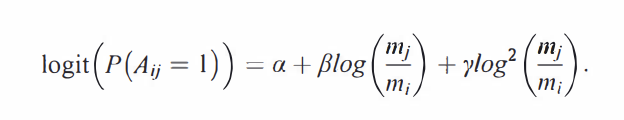
\includegraphics{figures/feeding_equ.png} (P(\(A_{1j}\) = 1) is the
probability predator i eats prey j).

\begin{enumerate}
\def\labelenumi{\alph{enumi}.}
\tightlist
\item
  Write a function and call it `probEat' to implement the equation
  above. Round the probability to two decimal places.
\end{enumerate}

Below are the values of alpha, beta, and gamma for the Serengeti. In
addition, you will need a function to compute the inverse logit function
because this equation is for the logit of the probability, so to
calculate the 0-1 probability you will need to take the inverse logit of
the other side of the equation. Also note, \(log^2\) is equivalent to
(log(\(m_i\)/\(m_j\)))\^{}2

\begin{Shaded}
\begin{Highlighting}[]
\NormalTok{alpha }\OtherTok{\textless{}{-}} \FloatTok{2.51}
\NormalTok{beta }\OtherTok{\textless{}{-}} \FloatTok{0.79}
\NormalTok{gamma }\OtherTok{\textless{}{-}} \SpecialCharTok{{-}}\FloatTok{0.37}
  
\NormalTok{inv\_logit }\OtherTok{\textless{}{-}} \ControlFlowTok{function}\NormalTok{(x) }\FunctionTok{exp}\NormalTok{(x)}\SpecialCharTok{/}\NormalTok{(}\DecValTok{1}\SpecialCharTok{+}\FunctionTok{exp}\NormalTok{(x))}
\end{Highlighting}
\end{Shaded}

\begin{Shaded}
\begin{Highlighting}[]
\NormalTok{probEat }\OtherTok{\textless{}{-}} \ControlFlowTok{function}\NormalTok{(mi, mj, alpha, beta, gamma) \{}
\NormalTok{  log\_squared }\OtherTok{\textless{}{-}} \FunctionTok{log}\NormalTok{(mj }\SpecialCharTok{/}\NormalTok{ mi)}\SpecialCharTok{\^{}}\DecValTok{2}
\NormalTok{  logit }\OtherTok{\textless{}{-}}\NormalTok{ alpha }\SpecialCharTok{+}\NormalTok{ beta }\SpecialCharTok{*} \FunctionTok{log}\NormalTok{(mj }\SpecialCharTok{/}\NormalTok{ mi) }\SpecialCharTok{+}\NormalTok{ gamma }\SpecialCharTok{*}\NormalTok{ log\_squared}
\NormalTok{  prob }\OtherTok{\textless{}{-}} \FunctionTok{inv\_logit}\NormalTok{(logit)}
  \FunctionTok{round}\NormalTok{(prob, }\DecValTok{2}\NormalTok{)}
\NormalTok{\}}

\NormalTok{mi }\OtherTok{\textless{}{-}} \DecValTok{10} 
\NormalTok{mj }\OtherTok{\textless{}{-}} \DecValTok{2}
\NormalTok{alpha }\OtherTok{\textless{}{-}} \FloatTok{2.51}
\NormalTok{beta }\OtherTok{\textless{}{-}} \FloatTok{0.79}
\NormalTok{gamma }\OtherTok{\textless{}{-}} \SpecialCharTok{{-}}\FloatTok{0.37}
\FunctionTok{probEat}\NormalTok{(mi, mj, alpha, beta, gamma)}
\end{Highlighting}
\end{Shaded}

\begin{verbatim}
## [1] 0.57
\end{verbatim}

\begin{enumerate}
\def\labelenumi{\alph{enumi}.}
\setcounter{enumi}{2}
\tightlist
\item
  Now create networks of who eats whom. We will start with adjacency
  matrices. We will assume all of our species are the size of females.
  For this step, don't worry about predators vs.~prey yet, just
  calculate all of the feeding probabilities based on body sizes.
\end{enumerate}

Hint: if you start with a square matrix of all zeros (one row and one
column for each species), you can use a for loop to fill in that matrix
with probabilities calculated from your function above.

\begin{Shaded}
\begin{Highlighting}[]
\NormalTok{adj\_matrix }\OtherTok{\textless{}{-}} \FunctionTok{matrix}\NormalTok{(}\DecValTok{0}\NormalTok{, }\AttributeTok{nrow =} \FunctionTok{nrow}\NormalTok{(sp\_mass), }\AttributeTok{ncol =} \FunctionTok{nrow}\NormalTok{(sp\_mass))}
\FunctionTok{rownames}\NormalTok{(adj\_matrix) }\OtherTok{\textless{}{-}}\NormalTok{ row\_labs\_sp}
\FunctionTok{colnames}\NormalTok{(adj\_matrix) }\OtherTok{\textless{}{-}}\NormalTok{ row\_labs\_sp}

\ControlFlowTok{for}\NormalTok{ (i }\ControlFlowTok{in} \DecValTok{1}\SpecialCharTok{:}\FunctionTok{nrow}\NormalTok{(adj\_matrix)) \{}
  \ControlFlowTok{for}\NormalTok{ (j }\ControlFlowTok{in} \DecValTok{1}\SpecialCharTok{:}\FunctionTok{ncol}\NormalTok{(adj\_matrix)) \{}
\NormalTok{    adj\_matrix[i, j] }\OtherTok{\textless{}{-}} \FunctionTok{probEat}\NormalTok{(sp\_mass}\SpecialCharTok{$}\NormalTok{f[j], sp\_mass}\SpecialCharTok{$}\NormalTok{f[i], alpha, beta, gamma)}
\NormalTok{  \}}
\NormalTok{\}}

\FunctionTok{head}\NormalTok{(adj\_matrix)}
\end{Highlighting}
\end{Shaded}

\begin{verbatim}
##                           Canis aureus Vulpes vulpes Lycaon pictus
## Canis aureus                      0.92          0.94          0.77
## Vulpes vulpes                     0.89          0.92          0.62
## Lycaon pictus                     0.95          0.95          0.92
## Hyaena hyaena                     0.95          0.94          0.94
## Crocuta crocuta                   0.94          0.91          0.95
## Panthera leo (long maned)         0.82          0.71          0.94
##                           Hyaena hyaena Crocuta crocuta
## Canis aureus                       0.65            0.42
## Vulpes vulpes                      0.46            0.22
## Lycaon pictus                      0.90            0.84
## Hyaena hyaena                      0.92            0.89
## Crocuta crocuta                    0.94            0.92
## Panthera leo (long maned)          0.94            0.95
##                           Panthera leo (long maned) Panthera leo (short maned)
## Canis aureus                                   0.04                       0.04
## Vulpes vulpes                                  0.01                       0.01
## Lycaon pictus                                  0.41                       0.41
## Hyaena hyaena                                  0.58                       0.58
## Crocuta crocuta                                0.76                       0.76
## Panthera leo (long maned)                      0.92                       0.92
##                           Panthera pardus Acinonyx jubatus Loxodonta africana
## Canis aureus                         0.30             0.49               0.00
## Vulpes vulpes                        0.14             0.28               0.00
## Lycaon pictus                        0.79             0.86               0.00
## Hyaena hyaena                        0.86             0.90               0.00
## Crocuta crocuta                      0.91             0.93               0.00
## Panthera leo (long maned)            0.95             0.95               0.05
##                           Equus asinus Equus grevyi Equus quagga
## Canis aureus                      0.00         0.00         0.01
## Vulpes vulpes                     0.00         0.00         0.00
## Lycaon pictus                     0.09         0.04         0.23
## Hyaena hyaena                     0.19         0.10         0.39
## Crocuta crocuta                   0.41         0.28         0.63
## Panthera leo (long maned)         0.84         0.78         0.90
##                           Diceros/Ceratotherium Sus scrofa
## Canis aureus                               0.00       0.57
## Vulpes vulpes                              0.00       0.36
## Lycaon pictus                              0.00       0.88
## Hyaena hyaena                              0.01       0.91
## Crocuta crocuta                            0.06       0.94
## Panthera leo (long maned)                  0.50       0.95
##                           Phacochoerus aethiopicus Hippopotamus amphibius
## Canis aureus                                  0.36                   0.00
## Vulpes vulpes                                 0.17                   0.00
## Lycaon pictus                                 0.81                   0.01
## Hyaena hyaena                                 0.87                   0.04
## Crocuta crocuta                               0.92                   0.13
## Panthera leo (long maned)                     0.95                   0.65
##                           Giraffa camelopardalis Dama mesopotamica
## Canis aureus                                0.00              0.09
## Vulpes vulpes                               0.00              0.03
## Lycaon pictus                               0.02              0.57
## Hyaena hyaena                               0.05              0.71
## Crocuta crocuta                             0.17              0.84
## Panthera leo (long maned)                   0.70              0.94
##                           Camelus dromedarius Taurotragus oryx
## Canis aureus                             0.00             0.00
## Vulpes vulpes                            0.00             0.00
## Lycaon pictus                            0.03             0.07
## Hyaena hyaena                            0.07             0.15
## Crocuta crocuta                          0.22             0.36
## Panthera leo (long maned)                0.74             0.82
##                           Tragelaphus spekei Addax nasomaculatus Oryx dammah
## Canis aureus                            0.42                0.22        0.03
## Vulpes vulpes                           0.22                0.09        0.01
## Lycaon pictus                           0.84                0.74        0.36
## Hyaena hyaena                           0.89                0.82        0.53
## Crocuta crocuta                         0.92                0.89        0.73
## Panthera leo (long maned)               0.95                0.95        0.92
##                           Oryx beisa Hippotragus equinus Kobus kob
## Canis aureus                    0.04                0.01      0.22
## Vulpes vulpes                   0.01                0.00      0.09
## Lycaon pictus                   0.44                0.14      0.74
## Hyaena hyaena                   0.60                0.27      0.82
## Crocuta crocuta                 0.78                0.52      0.89
## Panthera leo (long maned)       0.93                0.87      0.95
##                           Kobus megaceros Alcelaphus bucelaphus
## Canis aureus                         0.22                  0.04
## Vulpes vulpes                        0.09                  0.01
## Lycaon pictus                        0.74                  0.44
## Hyaena hyaena                        0.82                  0.60
## Crocuta crocuta                      0.89                  0.78
## Panthera leo (long maned)            0.95                  0.93
##                           Connochaetes taurinus Litocranius walleri
## Canis aureus                               0.03                0.57
## Vulpes vulpes                              0.01                0.36
## Lycaon pictus                              0.34                0.88
## Hyaena hyaena                              0.51                0.91
## Crocuta crocuta                            0.72                0.94
## Panthera leo (long maned)                  0.92                0.95
##                           Ammodorcas clarkei Gazella dorcas Gazella leptoceros
## Canis aureus                            0.70           0.81               0.83
## Vulpes vulpes                           0.52           0.69               0.72
## Lycaon pictus                           0.91           0.93               0.94
## Hyaena hyaena                           0.93           0.94               0.94
## Crocuta crocuta                         0.95           0.95               0.95
## Panthera leo (long maned)               0.94           0.93               0.92
##                           Gazella soemmerringii Capra ibex Ammotragus lervia
## Canis aureus                               0.45       0.30              0.42
## Vulpes vulpes                              0.24       0.14              0.22
## Lycaon pictus                              0.85       0.79              0.84
## Hyaena hyaena                              0.89       0.86              0.89
## Crocuta crocuta                            0.93       0.91              0.92
## Panthera leo (long maned)                  0.95       0.95              0.95
##                           Bos primigenius Syncerus caffer
## Canis aureus                         0.00            0.00
## Vulpes vulpes                        0.00            0.00
## Lycaon pictus                        0.00            0.11
## Hyaena hyaena                        0.00            0.22
## Crocuta crocuta                      0.02            0.46
## Panthera leo (long maned)            0.31            0.85
\end{verbatim}

\begin{enumerate}
\def\labelenumi{\alph{enumi}.}
\setcounter{enumi}{3}
\tightlist
\item
  Now that you have your matrix of potential feeding interactions based
  on body size, use the `carnivores' vector created above to set all of
  the feeding interactions of herbivores (0s in that vector) to zero. In
  foodwebs the columns are the higher trophic level and the rows are the
  lower. HINT: the function `sweep' may be useful, though there are many
  approaches to do the needed matrix multiplication. Print the row and
  column sums.
\end{enumerate}

\begin{Shaded}
\begin{Highlighting}[]
\NormalTok{adj\_matrix }\OtherTok{\textless{}{-}} \FunctionTok{sweep}\NormalTok{(adj\_matrix, }\DecValTok{2}\NormalTok{, carnivores, }\StringTok{\textasciigrave{}}\AttributeTok{*}\StringTok{\textasciigrave{}}\NormalTok{)}

\NormalTok{row\_sums }\OtherTok{\textless{}{-}} \FunctionTok{rowSums}\NormalTok{(adj\_matrix)}
\NormalTok{col\_sums }\OtherTok{\textless{}{-}} \FunctionTok{colSums}\NormalTok{(adj\_matrix)}

\FunctionTok{print}\NormalTok{(row\_sums)}
\end{Highlighting}
\end{Shaded}

\begin{verbatim}
##               Canis aureus              Vulpes vulpes 
##                       4.57                       3.55 
##              Lycaon pictus              Hyaena hyaena 
##                       7.03                       7.56 
##            Crocuta crocuta  Panthera leo (long maned) 
##                       8.02                       8.10 
## Panthera leo (short maned)            Panthera pardus 
##                       8.10                       8.17 
##           Acinonyx jubatus         Loxodonta africana 
##                       7.93                       3.34 
##               Equus asinus               Equus grevyi 
##                       7.36                       6.97 
##               Equus quagga      Diceros/Ceratotherium 
##                       7.84                       5.94 
##                 Sus scrofa   Phacochoerus aethiopicus 
##                       7.76                       8.11 
##     Hippopotamus amphibius     Giraffa camelopardalis 
##                       6.44                       6.63 
##          Dama mesopotamica        Camelus dromedarius 
##                       8.21                       6.78 
##           Taurotragus oryx         Tragelaphus spekei 
##                       7.20                       8.02 
##        Addax nasomaculatus                Oryx dammah 
##                       8.19                       8.05 
##                 Oryx beisa        Hippotragus equinus 
##                       8.14                       7.61 
##                  Kobus kob            Kobus megaceros 
##                       8.19                       8.19 
##      Alcelaphus bucelaphus      Connochaetes taurinus 
##                       8.14                       8.03 
##        Litocranius walleri         Ammodorcas clarkei 
##                       7.76                       7.37 
##             Gazella dorcas         Gazella leptoceros 
##                       6.70                       6.54 
##      Gazella soemmerringii                 Capra ibex 
##                       8.01                       8.17 
##          Ammotragus lervia            Bos primigenius 
##                       8.02                       5.27 
##            Syncerus caffer 
##                       7.45
\end{verbatim}

\begin{Shaded}
\begin{Highlighting}[]
\FunctionTok{print}\NormalTok{(col\_sums)}
\end{Highlighting}
\end{Shaded}

\begin{verbatim}
##               Canis aureus              Vulpes vulpes 
##                      28.74                      25.91 
##              Lycaon pictus              Hyaena hyaena 
##                      33.59                      33.99 
##            Crocuta crocuta  Panthera leo (long maned) 
##                      33.88                      29.91 
## Panthera leo (short maned)            Panthera pardus 
##                      29.91                      33.54 
##           Acinonyx jubatus         Loxodonta africana 
##                      33.99                       0.00 
##               Equus asinus               Equus grevyi 
##                       0.00                       0.00 
##               Equus quagga      Diceros/Ceratotherium 
##                       0.00                       0.00 
##                 Sus scrofa   Phacochoerus aethiopicus 
##                       0.00                       0.00 
##     Hippopotamus amphibius     Giraffa camelopardalis 
##                       0.00                       0.00 
##          Dama mesopotamica        Camelus dromedarius 
##                       0.00                       0.00 
##           Taurotragus oryx         Tragelaphus spekei 
##                       0.00                       0.00 
##        Addax nasomaculatus                Oryx dammah 
##                       0.00                       0.00 
##                 Oryx beisa        Hippotragus equinus 
##                       0.00                       0.00 
##                  Kobus kob            Kobus megaceros 
##                       0.00                       0.00 
##      Alcelaphus bucelaphus      Connochaetes taurinus 
##                       0.00                       0.00 
##        Litocranius walleri         Ammodorcas clarkei 
##                       0.00                       0.00 
##             Gazella dorcas         Gazella leptoceros 
##                       0.00                       0.00 
##      Gazella soemmerringii                 Capra ibex 
##                       0.00                       0.00 
##          Ammotragus lervia            Bos primigenius 
##                       0.00                       0.00 
##            Syncerus caffer 
##                       0.00
\end{verbatim}

\section{Lab part 2: Breaking the networks into time
periods}\label{lab-part-2-breaking-the-networks-into-time-periods}

\begin{enumerate}
\def\labelenumi{\alph{enumi}.}
\tightlist
\item
  With our matrix of feeding interaction we can create a web for each
  time period, including only the species that were not extinct in the
  period. Try first just using the second time period (the second column
  of `sp\_occ').
\end{enumerate}

Use the function `empty' from the bipartite package to empty the matrix
of rows and columns with no interactions. The number of species in the
second time period is 36 `sum(sp\_occ{[},2{]})'. Check to see that the
number of rows in your network with probabilities \textgreater{} 0 is
36.

HINT: You will need to zero out the rows where a species in not present
in that time period and the columns. The function `sweep' may be useful
again.

\begin{Shaded}
\begin{Highlighting}[]
\NormalTok{present\_species }\OtherTok{\textless{}{-}}\NormalTok{ sp\_occ[, }\DecValTok{2}\NormalTok{]}

\NormalTok{adj\_matrix\_time2 }\OtherTok{\textless{}{-}} \FunctionTok{sweep}\NormalTok{(adj\_matrix, }\DecValTok{1}\NormalTok{, present\_species, }\StringTok{\textasciigrave{}}\AttributeTok{*}\StringTok{\textasciigrave{}}\NormalTok{)}
\NormalTok{adj\_matrix\_time2 }\OtherTok{\textless{}{-}} \FunctionTok{sweep}\NormalTok{(adj\_matrix\_time2, }\DecValTok{2}\NormalTok{, present\_species, }\StringTok{\textasciigrave{}}\AttributeTok{*}\StringTok{\textasciigrave{}}\NormalTok{)}

\NormalTok{adj\_matrix\_time2 }\OtherTok{\textless{}{-}} \FunctionTok{empty}\NormalTok{(adj\_matrix\_time2)}

\NormalTok{num\_rows }\OtherTok{\textless{}{-}} \FunctionTok{nrow}\NormalTok{(adj\_matrix\_time2)}
\FunctionTok{print}\NormalTok{(num\_rows)}
\end{Highlighting}
\end{Shaded}

\begin{verbatim}
## [1] 36
\end{verbatim}

\begin{Shaded}
\begin{Highlighting}[]
\FunctionTok{head}\NormalTok{(adj\_matrix\_time2)}
\end{Highlighting}
\end{Shaded}

\begin{verbatim}
##                           Canis aureus Vulpes vulpes Lycaon pictus
## Canis aureus                      0.92          0.94          0.77
## Vulpes vulpes                     0.89          0.92          0.62
## Lycaon pictus                     0.95          0.95          0.92
## Hyaena hyaena                     0.95          0.94          0.94
## Crocuta crocuta                   0.94          0.91          0.95
## Panthera leo (long maned)         0.82          0.71          0.94
##                           Hyaena hyaena Crocuta crocuta
## Canis aureus                       0.65            0.42
## Vulpes vulpes                      0.46            0.22
## Lycaon pictus                      0.90            0.84
## Hyaena hyaena                      0.92            0.89
## Crocuta crocuta                    0.94            0.92
## Panthera leo (long maned)          0.94            0.95
##                           Panthera leo (long maned) Panthera leo (short maned)
## Canis aureus                                   0.04                       0.04
## Vulpes vulpes                                  0.01                       0.01
## Lycaon pictus                                  0.41                       0.41
## Hyaena hyaena                                  0.58                       0.58
## Crocuta crocuta                                0.76                       0.76
## Panthera leo (long maned)                      0.92                       0.92
##                           Panthera pardus
## Canis aureus                         0.30
## Vulpes vulpes                        0.14
## Lycaon pictus                        0.79
## Hyaena hyaena                        0.86
## Crocuta crocuta                      0.91
## Panthera leo (long maned)            0.95
\end{verbatim}

\begin{enumerate}
\def\labelenumi{\alph{enumi}.}
\setcounter{enumi}{1}
\tightlist
\item
  Now create a network for all of the time points by creating a list
  where each element is a network. You will need to use a for loop, or
  an `lapply' if you feel like experimenting with apply functions. Print
  the first 5 columns and rows of the 5th time period.
\end{enumerate}

HINT: If choosing the for loop route, remember to create an empty list
of a specific length use the function `vector'. To access a specific
element of a list, use {[}{[}{]}{]}, for example cool\_list{[}{[}1{]}{]}
accesses the first element of the list.

\begin{Shaded}
\begin{Highlighting}[]
\NormalTok{all\_time\_webs }\OtherTok{\textless{}{-}} \FunctionTok{vector}\NormalTok{(}\StringTok{"list"}\NormalTok{, }\FunctionTok{ncol}\NormalTok{(sp\_occ))}

\CommentTok{\# Loop through the time periods (columns of sp\_occ)}
\ControlFlowTok{for}\NormalTok{ (time\_period }\ControlFlowTok{in} \DecValTok{1}\SpecialCharTok{:}\FunctionTok{ncol}\NormalTok{(sp\_occ)) \{}
  \CommentTok{\# Extract the species present in the current time period}
\NormalTok{  present\_species }\OtherTok{\textless{}{-}}\NormalTok{ sp\_occ[, time\_period]}
  
  \CommentTok{\# Zero out rows and columns for species not present in the time period}
\NormalTok{  adj\_matrix\_time }\OtherTok{\textless{}{-}} \FunctionTok{sweep}\NormalTok{(adj\_matrix, }\DecValTok{1}\NormalTok{, present\_species, }\StringTok{\textasciigrave{}}\AttributeTok{*}\StringTok{\textasciigrave{}}\NormalTok{)}
\NormalTok{  adj\_matrix\_time }\OtherTok{\textless{}{-}} \FunctionTok{sweep}\NormalTok{(adj\_matrix\_time, }\DecValTok{2}\NormalTok{, present\_species, }\StringTok{\textasciigrave{}}\AttributeTok{*}\StringTok{\textasciigrave{}}\NormalTok{)}
  
  \CommentTok{\# Store the filtered adjacency matrix (network) in the list}
\NormalTok{  all\_time\_webs[[time\_period]] }\OtherTok{\textless{}{-}}\NormalTok{ adj\_matrix\_time}
\NormalTok{\}}
\FunctionTok{head}\NormalTok{(all\_time\_webs[[}\DecValTok{5}\NormalTok{]], }\DecValTok{5}\NormalTok{)}
\end{Highlighting}
\end{Shaded}

\begin{verbatim}
##                 Canis aureus Vulpes vulpes Lycaon pictus Hyaena hyaena
## Canis aureus            0.92          0.94          0.77          0.65
## Vulpes vulpes           0.89          0.92          0.62          0.46
## Lycaon pictus           0.95          0.95          0.92          0.90
## Hyaena hyaena           0.95          0.94          0.94          0.92
## Crocuta crocuta         0.00          0.00          0.00          0.00
##                 Crocuta crocuta Panthera leo (long maned)
## Canis aureus                  0                      0.04
## Vulpes vulpes                 0                      0.01
## Lycaon pictus                 0                      0.41
## Hyaena hyaena                 0                      0.58
## Crocuta crocuta               0                      0.00
##                 Panthera leo (short maned) Panthera pardus Acinonyx jubatus
## Canis aureus                          0.04            0.30                0
## Vulpes vulpes                         0.01            0.14                0
## Lycaon pictus                         0.41            0.79                0
## Hyaena hyaena                         0.58            0.86                0
## Crocuta crocuta                       0.00            0.00                0
##                 Loxodonta africana Equus asinus Equus grevyi Equus quagga
## Canis aureus                     0            0            0            0
## Vulpes vulpes                    0            0            0            0
## Lycaon pictus                    0            0            0            0
## Hyaena hyaena                    0            0            0            0
## Crocuta crocuta                  0            0            0            0
##                 Diceros/Ceratotherium Sus scrofa Phacochoerus aethiopicus
## Canis aureus                        0          0                        0
## Vulpes vulpes                       0          0                        0
## Lycaon pictus                       0          0                        0
## Hyaena hyaena                       0          0                        0
## Crocuta crocuta                     0          0                        0
##                 Hippopotamus amphibius Giraffa camelopardalis Dama mesopotamica
## Canis aureus                         0                      0                 0
## Vulpes vulpes                        0                      0                 0
## Lycaon pictus                        0                      0                 0
## Hyaena hyaena                        0                      0                 0
## Crocuta crocuta                      0                      0                 0
##                 Camelus dromedarius Taurotragus oryx Tragelaphus spekei
## Canis aureus                      0                0                  0
## Vulpes vulpes                     0                0                  0
## Lycaon pictus                     0                0                  0
## Hyaena hyaena                     0                0                  0
## Crocuta crocuta                   0                0                  0
##                 Addax nasomaculatus Oryx dammah Oryx beisa Hippotragus equinus
## Canis aureus                      0           0          0                   0
## Vulpes vulpes                     0           0          0                   0
## Lycaon pictus                     0           0          0                   0
## Hyaena hyaena                     0           0          0                   0
## Crocuta crocuta                   0           0          0                   0
##                 Kobus kob Kobus megaceros Alcelaphus bucelaphus
## Canis aureus            0               0                     0
## Vulpes vulpes           0               0                     0
## Lycaon pictus           0               0                     0
## Hyaena hyaena           0               0                     0
## Crocuta crocuta         0               0                     0
##                 Connochaetes taurinus Litocranius walleri Ammodorcas clarkei
## Canis aureus                        0                   0                  0
## Vulpes vulpes                       0                   0                  0
## Lycaon pictus                       0                   0                  0
## Hyaena hyaena                       0                   0                  0
## Crocuta crocuta                     0                   0                  0
##                 Gazella dorcas Gazella leptoceros Gazella soemmerringii
## Canis aureus                 0                  0                     0
## Vulpes vulpes                0                  0                     0
## Lycaon pictus                0                  0                     0
## Hyaena hyaena                0                  0                     0
## Crocuta crocuta              0                  0                     0
##                 Capra ibex Ammotragus lervia Bos primigenius Syncerus caffer
## Canis aureus             0                 0               0               0
## Vulpes vulpes            0                 0               0               0
## Lycaon pictus            0                 0               0               0
## Hyaena hyaena            0                 0               0               0
## Crocuta crocuta          0                 0               0               0
\end{verbatim}

\section{Lab part 3: Visualize the
networks}\label{lab-part-3-visualize-the-networks}

\begin{enumerate}
\def\labelenumi{\alph{enumi}.}
\tightlist
\item
  Convert the adjacency matrices to igraph class objects using the
  function `graph\_from\_adjacency\_matrix'. You can use a for loop or
  an lapply. Because these are food webs, set the argument mode to
  ``directed'' and the argument diag to FALSE (this means a species
  cannot consumer members of its own species, i.e., no
  canabalism/self-loops). Also remember that these interactions are
  weighted.
\end{enumerate}

\begin{Shaded}
\begin{Highlighting}[]
\CommentTok{\# Initialize an empty list to store the igraph objects for each time period}
\NormalTok{igraph\_networks }\OtherTok{\textless{}{-}} \FunctionTok{vector}\NormalTok{(}\StringTok{"list"}\NormalTok{, }\FunctionTok{length}\NormalTok{(all\_time\_webs))}

\CommentTok{\# Convert each adjacency matrix to an igraph object}
\ControlFlowTok{for}\NormalTok{ (time\_period }\ControlFlowTok{in} \DecValTok{1}\SpecialCharTok{:}\FunctionTok{length}\NormalTok{(all\_time\_webs)) \{}
  \CommentTok{\# Convert the adjacency matrix to a directed, weighted igraph object}
\NormalTok{  igraph\_networks[[time\_period]] }\OtherTok{\textless{}{-}} \FunctionTok{graph\_from\_adjacency\_matrix}\NormalTok{(}
\NormalTok{    all\_time\_webs[[time\_period]], }
    \AttributeTok{mode =} \StringTok{"directed"}\NormalTok{, }
    \AttributeTok{diag =} \ConstantTok{FALSE}\NormalTok{, }
    \AttributeTok{weighted =} \ConstantTok{TRUE}
\NormalTok{  )}
\NormalTok{\}}

\NormalTok{igraph\_networks[[}\DecValTok{5}\NormalTok{]]}
\end{Highlighting}
\end{Shaded}

\begin{verbatim}
## IGRAPH 5cf80e1 DNW- 39 208 -- 
## + attr: name (v/c), weight (e/n)
## + edges from 5cf80e1 (vertex names):
##  [1] Canis aureus ->Vulpes vulpes             
##  [2] Canis aureus ->Lycaon pictus             
##  [3] Canis aureus ->Hyaena hyaena             
##  [4] Canis aureus ->Panthera leo (long maned) 
##  [5] Canis aureus ->Panthera leo (short maned)
##  [6] Canis aureus ->Panthera pardus           
##  [7] Vulpes vulpes->Canis aureus              
##  [8] Vulpes vulpes->Lycaon pictus             
## + ... omitted several edges
\end{verbatim}

\begin{enumerate}
\def\labelenumi{\alph{enumi}.}
\setcounter{enumi}{1}
\tightlist
\item
  Plot three networks of your choice, using different colors for the
  predators and prey.
\end{enumerate}

\begin{Shaded}
\begin{Highlighting}[]
\NormalTok{carnivore\_colors }\OtherTok{\textless{}{-}} \FunctionTok{ifelse}\NormalTok{(carnivores }\SpecialCharTok{==} \DecValTok{1}\NormalTok{, }\StringTok{"red"}\NormalTok{, }\StringTok{"green"}\NormalTok{)}

\CommentTok{\# Plot the first network (choose a time period, e.g., 1st)}
\NormalTok{plot\_g1 }\OtherTok{\textless{}{-}} \ControlFlowTok{function}\NormalTok{() \{}
  \CommentTok{\# Choose the first time period network (or any other you prefer)}
\NormalTok{  g1 }\OtherTok{\textless{}{-}}\NormalTok{ igraph\_networks[[}\DecValTok{1}\NormalTok{]]}
  
  \CommentTok{\# Plot with different colors for predators and prey}
  \FunctionTok{plot}\NormalTok{(g1, }
       \AttributeTok{vertex.color =}\NormalTok{ carnivore\_colors, }
       \AttributeTok{vertex.size =} \DecValTok{15}\NormalTok{, }
       \AttributeTok{vertex.label.cex =} \FloatTok{0.8}\NormalTok{, }
       \AttributeTok{edge.arrow.size =} \FloatTok{0.5}\NormalTok{, }
       \AttributeTok{main =} \StringTok{"Network for Time Period 1"}\NormalTok{)}
\NormalTok{\}}

\CommentTok{\# Plot the second network (choose the 5th time period)}
\NormalTok{plot\_g2 }\OtherTok{\textless{}{-}} \ControlFlowTok{function}\NormalTok{() \{}
  \CommentTok{\# Choose the fifth time period network}
\NormalTok{  g2 }\OtherTok{\textless{}{-}}\NormalTok{ igraph\_networks[[}\DecValTok{5}\NormalTok{]]}
  
  \CommentTok{\# Plot with different colors for predators and prey}
  \FunctionTok{plot}\NormalTok{(g2, }
       \AttributeTok{vertex.color =}\NormalTok{ carnivore\_colors, }
       \AttributeTok{vertex.size =} \DecValTok{15}\NormalTok{, }
       \AttributeTok{vertex.label.cex =} \FloatTok{0.8}\NormalTok{, }
       \AttributeTok{edge.arrow.size =} \FloatTok{0.5}\NormalTok{, }
       \AttributeTok{main =} \StringTok{"Network for Time Period 5"}\NormalTok{)}
\NormalTok{\}}

\CommentTok{\# Plot the third network (choose the 10th time period)}
\NormalTok{plot\_g3 }\OtherTok{\textless{}{-}} \ControlFlowTok{function}\NormalTok{() \{}
  \CommentTok{\# Choose the tenth time period network}
\NormalTok{  g3 }\OtherTok{\textless{}{-}}\NormalTok{ igraph\_networks[[}\DecValTok{10}\NormalTok{]]}
  \FunctionTok{plot}\NormalTok{(g3, }
       \AttributeTok{vertex.color =}\NormalTok{ carnivore\_colors, }
       \AttributeTok{vertex.size =} \DecValTok{15}\NormalTok{, }
       \AttributeTok{vertex.label.cex =} \FloatTok{0.8}\NormalTok{, }
       \AttributeTok{edge.arrow.size =} \FloatTok{0.5}\NormalTok{, }
       \AttributeTok{main =} \StringTok{"Network for Time Period 10"}\NormalTok{)}
\NormalTok{\}}

\FunctionTok{plot\_g1}\NormalTok{()}
\end{Highlighting}
\end{Shaded}

\includegraphics{6-lab-foodwebs_files/figure-latex/plot-g1-1.pdf}

\begin{Shaded}
\begin{Highlighting}[]
\FunctionTok{plot\_g2}\NormalTok{()}
\end{Highlighting}
\end{Shaded}

\includegraphics{6-lab-foodwebs_files/figure-latex/plot-g2-1.pdf}

\begin{Shaded}
\begin{Highlighting}[]
\FunctionTok{plot\_g3}\NormalTok{()}
\end{Highlighting}
\end{Shaded}

\includegraphics{6-lab-foodwebs_files/figure-latex/plot-g3-1.pdf}

\end{document}
